\section{SG\_\-File Class Reference}
\label{class_s_g___file}\index{SG_File@{SG\_\-File}}
This is a generic class for creating a file with the solar system description.  


{\tt \#include $<$SG\_\-File.h$>$}

Inheritance diagram for SG\_\-File::\begin{figure}[H]
\begin{center}
\leavevmode
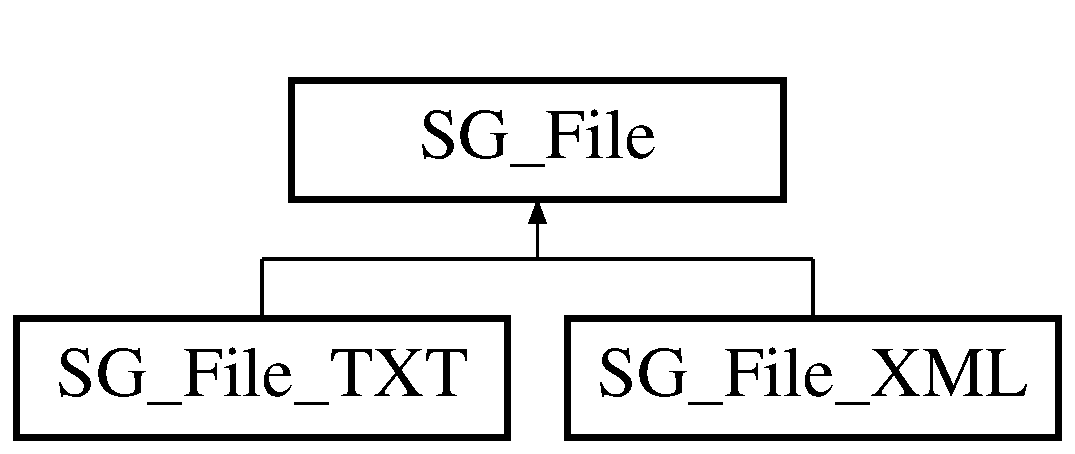
\includegraphics[height=2cm]{class_s_g___file}
\end{center}
\end{figure}
\subsection*{Public Member Functions}
\begin{CompactItemize}
\item 
{\bf SG\_\-File} (SG\_\-String filename, long seed)\label{class_s_g___file_a0}

\begin{CompactList}\small\item\em Constructor. \item\end{CompactList}\item 
virtual {\bf $\sim$SG\_\-File} ()\label{class_s_g___file_a1}

\begin{CompactList}\small\item\em Destructor. Close the output file. \item\end{CompactList}\item 
void {\bf write\-Star\-Description} ({\bf SG\_\-Star} $\ast$star)\label{class_s_g___file_a2}

\begin{CompactList}\small\item\em Write all the data concerning the Star, in the file. \item\end{CompactList}\item 
void {\bf write\-Planet\-Description} ({\bf SG\_\-Planet} $\ast$planet)\label{class_s_g___file_a3}

\begin{CompactList}\small\item\em Write all the data concerning the Planet, in the file. \item\end{CompactList}\end{CompactItemize}
\subsection*{Protected Member Functions}
\begin{CompactItemize}
\item 
void {\bf write\-Planet} ({\bf SG\_\-Planet} $\ast$planet)\label{class_s_g___file_b1}

\begin{CompactList}\small\item\em write the Planet description \item\end{CompactList}\item 
void {\bf write\-Solid\-Planet} ({\bf SG\_\-Planet} $\ast$planet)\label{class_s_g___file_b2}

\begin{CompactList}\small\item\em write the planet description for solid planets \item\end{CompactList}\item 
void {\bf write\-Gas\-Planet} ({\bf SG\_\-Planet} $\ast$planet)
\begin{CompactList}\small\item\em Write data for gas planets. \item\end{CompactList}\item 
void {\bf write\-Climate} ({\bf SG\_\-Planet} $\ast$planet)\label{class_s_g___file_b4}

\begin{CompactList}\small\item\em Write the planet description for solid planets. \item\end{CompactList}\item 
void {\bf write\-Atmosphere} ({\bf SG\_\-Planet} $\ast$planet)\label{class_s_g___file_b5}

\begin{CompactList}\small\item\em Write the atmosphere data. \item\end{CompactList}\end{CompactItemize}


\subsection{Detailed Description}
This is a generic class for creating a file with the solar system description. 

This class must be instancied into derived classes. For instance derived class {\bf SG\_\-File\_\-TXT}{\rm (p.\,\pageref{class_s_g___file___t_x_t})} to produce a Text file, {\bf SG\_\-File\_\-XML}{\rm (p.\,\pageref{class_s_g___file___x_m_l})} to produce an XML file, and based on these examples, others derived classes can be created, and used in {\bf SG\_\-Solar\-System}{\rm (p.\,\pageref{class_s_g___solar_system})}. 



\subsection{Member Function Documentation}
\index{SG_File@{SG\_\-File}!writeGasPlanet@{writeGasPlanet}}
\index{writeGasPlanet@{writeGasPlanet}!SG_File@{SG\_\-File}}
\subsubsection{\setlength{\rightskip}{0pt plus 5cm}void SG\_\-File::write\-Gas\-Planet ({\bf SG\_\-Planet} $\ast$ {\em planet})\hspace{0.3cm}{\tt  [protected]}}\label{class_s_g___file_b3}


Write data for gas planets. 

Note: I use Planet::calculate\-Pressure to determine the pressure inside the gas planet. This is a not a very good approximation. 

The documentation for this class was generated from the following files:\begin{CompactItemize}
\item 
E:/sphinx/LFE/lib\_\-stargen/SG\_\-File.h\item 
E:/sphinx/LFE/lib\_\-stargen/SG\_\-File.cpp\end{CompactItemize}
